\scanpage{21}
\mspage{20}
\begin{center}
U N I V E R S I T E\\
DES SCIENCES ET TECHNIQUES\\
DU LANGUEDOC\\
------------\\
Service de la Scolarité\\
MR/IE\\
\uline{Diffusion} : Liste A\\
N$^\circ$ 2090
\end{center}
Montpellier, le 2 avril 1980

\begin{center}
\uline{AVIS DE SOUTENANCE D'UNE THESE DE DOCTORAT DE SPECIALITE} :\\
\uline{CHIMIE ORGANIQUE PHYSIQUE}
\end{center}
\uline{Nom et Prénom} : MARCHETTI Jacqueline épouse SMADJA

\uline{Titre de la thèse} : Résolution cinétique et détermination du pouvoir rotatoire spécifique
de cétones chirales

\uline{Date, heure et lieu de soutenance prévus} : 10 avril 1980 à 10 heures ; U.E.R. des Sciences,
Centre Universitaire de la Réunion

\uline{Nom du Directeur de la thèse} : Messieurs Gérard LAMATY et Jacques CONAN

\uline{Désignation du laboratoire où la thèse est préparée} :
Laboratoire de Chimie Organique Centre Universitaire de la Réunion

\uline{Analyse de l'ouvrage} :
Un certain nombre de dioxolannes-1,3 diastéréoisomères ont été synthétisés à partir de cétones
chirales et de diols optiquement actifs dérivés de l'acide R-R tartrique.

Les constantes de vitesse d'hydrolyse de ces dioxolannes ont été mesurées ainsi que l'évolu-
tion, en fonction du temps, du pouvoir rotatoire de la cétone obtenue. A partir de ces deux
données on déduit le pouvoir rotatoire spécifique des cétones et les meilleures conditions
d'obtention de produits optiquement actifs.

\uline{Durée approximative des recherches ayant abouti à la thèse} : 4 ans.

\uline{Composition du jury proposé} : MM. : LAMATY Gérard\\
LATTES Armand\\
CARBONEL Max\\
ROQUE J.P.\\
CONAN Jacques

P/le Secrétaire Général\\
L'Attachée d'Administration Universitaire,

\figure{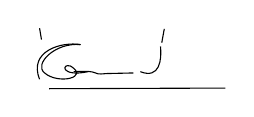
\begin{tikzpicture}[x=.8cm,y=.8cm]
\draw (0,.1) .. controls (-.18,.55) and (.35,.7) .. (.65,.65);
\draw (.65,.65) .. controls (.25,.69) and (-.1,.34) .. (.08,.2) .. controls (.3,.01) and (.8,.13) .. (.49,.31) .. controls (.35,.36) and (.33,.13) .. (.77,.22);
\draw (.54,.22) .. controls (1,.25) and (.8,.16) .. (1.05,.19)--(1.49,.2);
\draw (1.6,.22) .. controls (1.91,.1) and (1.94,.41) .. (1.92,.62);
\draw (1.94,.68)--(1.98,.9);
\draw (.03,.73)--(0,.91);
\draw (.15,-.05)--(2.95,-.04);
\end{tikzpicture}}
\uline{A. GENTIL.}

MR LE PROFESSEUR GROTHENDIECK ALEX.

MATHEMATIQUES\hfill 5
